\section{Introduction}

Whether animals other than human beings possess languages has long been a 
contentious scientific topic \citet{snowdon1990language}, with debates revolving around whether 
animal communications contains regular lexicon, grammar and semantics \citet{rendall2021aping}. 
Better understanding of animal languages can significantly contribute to animal
welfare, agriculture, disaster control, resource extraction and ultimately
understanding of our planet. To date, the research on animal communications
has been hindered by lack of quality data. Audio recordings of animal
communications, especially by amateurs, are often laced with 
background noise and interferences, which poses significant obstacles 
to the advancement of this research endeavor. Currently, there is no available interactive system, 
but such a system is crucial for researchers to directly and visually 
observe and compare the connections and differences between animal vocalization segments.

We chose dogs as our research subjects due to their widespread integration into human society, with many people keeping dogs as pets. However, even so, we had to make trade-offs in terms of the generality and accuracy of the data. Accurate, low-noise dog videos recorded with sophisticated equipment are rare, let alone videos of other animals that humans encounter less frequently. However, large datasets often come with a compromise in terms of the presence of noise or audio quality.

Furthermore, evaluating the transcription results of canine language poses a challenging task. Without a ground truth for canine language, we can only infer the performance of the transcription results through observations, listening, comparing the consistency of canine sounds, and their occurrence contexts. To facilitate researchers in conveniently and thoroughly studying canine language transcription, we have introduced for the first time an interactive and scalable canine lexical discovery system \footnote{The demo is available at \url{http://202.120.38.146:8079/}}.

The system is an interactive and scalable canine sound transcription and vocabulary discovery system. In addition to transcribing canine sounds into symbolic sequences as shown as \figref{fig:intro1}, the system also provides clickable functionality for listening to canine sound phonemes, facilitating users or researchers in identifying the consistency of the same phonemes in canine sounds. Furthermore, the system can continue to expand its transcription methods beyond our proposed baseline method, allowing for the adoption of more accurate and efficient methods in the future.

\begin{figure}[th]
    \centering
    \scalebox{0.55}{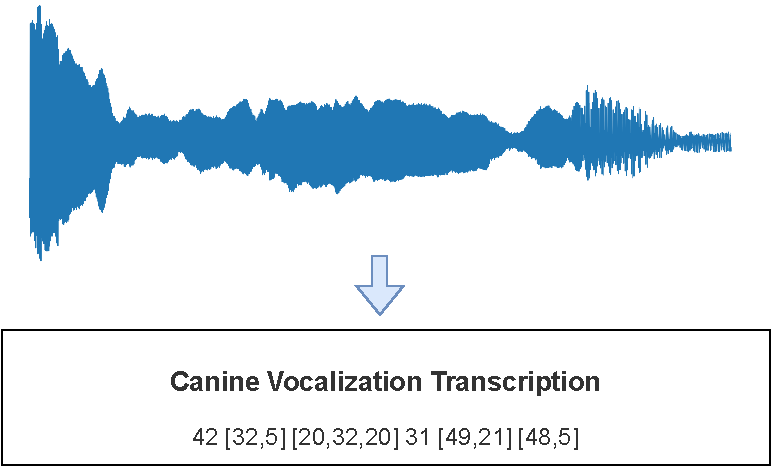
\includegraphics{introp1.pdf}}
	\caption{Canine vocalization Transcription Example}
    \label{fig:intro1}
\end{figure}




Additionally, the platform can present a two-dimensional mapping of cluster centers for canine phoneme audio along with audio examples, aiding users or researchers in exploring the relationships between phonemes with similar sound characteristics and the accuracy of phoneme classification. To further analyze the meaning of canine language, the platform also provides a canine vocabulary derived from NLP techniques along with corresponding video and audio examples, facilitating researchers in observing, distinguishing, and validating the relationships between canine words and environmental or situational contexts. Overall, the system is an intuitive canine sound transcription platform that is ready-to-use and scalable, designed for researchers, enabling them to verify the accuracy of each step in the transcription process through a visual canine word discovery system.

This paper presents a canine language lexical analysis system, our contributions include:
%\KZ{These bullets are too verbose and hard to understand.} \MY{you can boldly say that this is the first interactive animal language segmentation and analysis system, that allows xxx. the 1st point should be about what you did; 2nd point is what features it has; 3rd can be the evaluation. currently the 2nd and 3rd point feels they can go into previous paragraphs where you persuad your readers, but they are not contributions.}
\begin{itemize}
	% \item We designed and implemented an interactive platform for transcribing dog videos or audio files, showcasing preliminary dog language phonemes and vocabulary.
	\item We designed and implemented the first interactive animal language segmentation and analysis system, that allows transcribing dog videos or audio files, demonstrating preliminary dog language phonemes and vocabulary.
	% \item The platform provides a useful tool for validating whether dogs possess fixed language patterns and aids scholars in better understanding the relationship between dog vocalizations and behavior.
	\item This interactive and scalable system provides users with the functionality to upload their own recorded canine video or audio files and validate their relationship with the environment, actions, and consistency of canine vocalizations.
	% \item The platform will continue to serve as an analytical tool for exploring the meaning of dog language, the connection between dog vocalization words and scenarios, and other related research. It will aid scholars in systematically segmenting and transcribing dog vocalizations, laying important groundwork for future studies.
	\item The phonemes obtained through our proposed pipeline exhibit significant consistency in acoustic features. The words discovered in the vocabulary demonstrate basic temporal characteristics typical of regular words. Additionally, the quality of some transcriptions has been validated as excellent.
\end{itemize}
